%%%%%%%%%%%%%%%%%%%%%%%%%%%%%%%%%%%%%%%%%
% Short Sectioned Assignment LaTeX Template Version 1.0 (5/5/12)
% This template has been downloaded from: http://www.LaTeXTemplates.com
% Original author:  Frits Wenneker (http://www.howtotex.com)
% License: CC BY-NC-SA 3.0 (http://creativecommons.org/licenses/by-nc-sa/3.0/)
%%%%%%%%%%%%%%%%%%%%%%%%%%%%%%%%%%%%%%%%%

%----------------------------------------------------------------------------------------
%	PACKAGES AND OTHER DOCUMENT CONFIGURATIONS
%----------------------------------------------------------------------------------------

\documentclass[paper=a4, fontsize=11pt]{scrartcl} % A4 paper and 11pt font size

% ---- Entrada y salida de texto -----

\usepackage[T1]{fontenc} % Use 8-bit encoding that has 256 glyphs
\usepackage[utf8]{inputenc}
%\usepackage{fourier} % Use the Adobe Utopia font for the document - comment this line to return to the LaTeX default


\usepackage[utf8]{inputenc}
\usepackage[T1]{fontenc}
\usepackage[spanish]{babel}
\usepackage{times}

\usepackage{color}
\definecolor{gray97}{gray}{.97}
\definecolor{gray75}{gray}{.75}
\definecolor{gray45}{gray}{.45}

\usepackage{listings}
\lstset{ frame=Ltb,
	framerule=0pt,
	aboveskip=0.5cm,
	framextopmargin=3pt,
	framexbottommargin=3pt,
	framexleftmargin=0.4cm,
	framesep=0pt,
	rulesep=.4pt,
	backgroundcolor=\color{gray97},
	rulesepcolor=\color{black},
	%
	stringstyle=\ttfamily,
	showstringspaces = false,
	basicstyle=\small\ttfamily,
	commentstyle=\color{gray45},
	keywordstyle=\bfseries,
	%
	numbers=left,
	numbersep=15pt,
	numberstyle=\tiny,
	numberfirstline = false,
	breaklines=true,
}

% minimizar fragmentado de listados
\lstnewenvironment{listing}[1][]
{\lstset{#1}\pagebreak[0]}{\pagebreak[0]}

\lstdefinestyle{consola}
{basicstyle=\scriptsize\bf\ttfamily,
	backgroundcolor=\color{gray75},
}

\lstdefinestyle{C}
{language=C,
}
% ---- Idioma --------

\usepackage[spanish, es-tabla]{babel} % Selecciona el español para palabras introducidas automáticamente, p.ej. "septiembre" en la fecha y especifica que se use la palabra Tabla en vez de Cuadro
% ---- Otros paquetes ----

\usepackage{amsmath,amsfonts,amsthm} % Math packages
%\usepackage{graphics,graphicx, floatrow} %para incluir imágenes y notas en las imágenes
\usepackage{graphics,graphicx, float} %para incluir imágenes y colocarlas

% Para hacer tablas comlejas
%\usepackage{multirow}
%\usepackage{threeparttable}

%\usepackage{sectsty} % Allows customizing section commands
%\allsectionsfont{\centering \normalfont\scshape} % Make all sections centered, the default font and small caps

\usepackage{fancyhdr} % Custom headers and footers
\pagestyle{fancyplain} % Makes all pages in the document conform to the custom headers and footers
\fancyhead{} % No page header - if you want one, create it in the same way as the footers below
\fancyfoot[L]{} % Empty left footer
\fancyfoot[C]{} % Empty center footer
\fancyfoot[R]{\thepage} % Page numbering for right footer
\renewcommand{\headrulewidth}{0pt} % Remove header underlines
\renewcommand{\footrulewidth}{0pt} % Remove footer underlines
\setlength{\headheight}{13.6pt} % Customize the height of the header

\numberwithin{equation}{section} % Number equations within sections (i.e. 1.1, 1.2, 2.1, 2.2 instead of 1, 2, 3, 4)
\numberwithin{figure}{section} % Number figures within sections (i.e. 1.1, 1.2, 2.1, 2.2 instead of 1, 2, 3, 4)
\numberwithin{table}{section} % Number tables within sections (i.e. 1.1, 1.2, 2.1, 2.2 instead of 1, 2, 3, 4)

\setlength\parindent{0pt} % Removes all indentation from paragraphs - comment this line for an assignment with lots of text

\newcommand{\horrule}[1]{\rule{\linewidth}{#1}} % Create horizontal rule command with 1 argument of height


\begin{document}
\title{
\normalfont \normalsize 
\textsc{{\bf Metaheurísticas (2015-16) \\ Grado en Ingeniería Informática \\ Universidad de Granada} \\ [25pt] % Your university, school and/or department name(s)
\horrule{0.5pt} \\[0.4cm] % Thin top horizontal rule
\huge Práctica 4: Optimización basada en colonias de hormigas para la selección de características\\ % The assignment title
\horrule{2pt} \\[0.5cm] % Thick bottom horizontal rule
}}
\author{Miguel López Campos\\ 54120359W\\ miguelberja@correo.ugr.es\\ Grupo Viernes 18:30} % Nombre y apellidos


\date{\normalsize\today} % Incluye la fecha actual
%----------------------------------------------------------------------------------------
% DOCUMENTO
%----------------------------------------------------------------------------------------


	
	\maketitle % Muestra el Título
	\newpage %inserta un salto de página
	
	\tableofcontents % para generar el índice de contenidos
	\listoffigures

	
	\newpage
	
	\
	
	
	
	\section{Descripción del problema}
	El problema que estamos abordando es la selección de características. Este problema es muy útil en el campo de "machine learning".
	\\
	\\
	Tenemos un conjunto de datos de entrenamiento y otro de validación, ambos etiquetados o clasificados. Lo que queremos hacer es 'aprender' una función que a partir de las características del conjunto de datos de entrenamiento, nos permita estimar el etiquetado de otros vectores de características. Lo que nosotros queremos hacer es eliminar las características que no son relevantes en el problema, eliminando de esta manera ruido en el conjunto de datos y mejorando la eficiencia de nuestro clasificador. Es decir, no sólo mejoraremos el tiempo, si no muy probablemente la calidad de nuestras soluciones también (en cuanto al error se refiere).
	\\
	\\
	La gran dificultad de este problema radica en el gran número de soluciones posibles, llevándonos al punto de que un algoritmo Greedy que nos garantice la solución óptima podría llevarnos días de ejecución para determinados problemas. Es por esto por lo que tenemos que usar Metaheurísticas. Necesitamos soluciones buenas (aunque no sea la mejor) en un tiempo menor.
	\\
	\\
	Nosotros usaremos para clasificar el algoritmo 3NN. Lo que hace este algoritmo es calcular la distancia euclídea entre el vector de características al cual queremos estimar una clase y el resto de vectores de características del conjunto de entrenamiento. Lo que hace el 3NN es coger los 3 elementos menos distantes y la clase mayoritaria entre esos 3 será la estimación que haremos.
	\\
	\\
	Validaremos con la técnica 5x2 Cross Validation. Usaremos 5 particiones de los datos distintas al 50\% (y aleatorias) y aprenderemos el clasificador con una submuestra y validaremos con la otra y después al contrario. Con esta técnica tendremos el porcentaje de acierto, que nos servirá para ver la calidad de nuestro algoritmo.
	\\
	\\
	Otros datos con los que valoraremos la calidad de nuestros algoritmos serán los tiempos de ejeución y los porcentajes de reducción, es decir, el porcentaje de características que hemos reducido.
	\\
	\\
	Con nuestras metaheurísticas querremos optimizar la función de acierto. Es decir, queremos maximizar el acierto, siendo la función:\\
	$tasaclass = 100*\frac{nºinstancias bien clasificadas}{nº instancias Total}$
	
	\newpage
	
	
	\section{Descripción de los aspectos comunes de los algoritmos}
	La práctica ha sido desarrollada en C++.
	\\
	
	\begin{enumerate}
		\item Representación de las soluciones. Para representar las soluciones utilizaremos un array de booleanos. Será común a todos los algoritmos. Si la componente $i$ es true, esto indicará que la característica $i$ se tendrá en cuenta (no ha sido eliminada).
		
		\item Función objetivo. La función que queremos optimizar se trata del porcentaje de acierto de estimaciones de clases, descrita en el apartado anterior.
		\\
		\\
		En pseudocódigo es la siguiente:
		\begin{lstlisting}
funcion_objetivo(conjunto_training, caracteristicas_activas)
begin
  Para todo elemento i del conjunto_test
  begin
    elemento <- elemento i del conjunto_training
	clase <- 3NN(conjunto_training-{elemento}, elemento, caracteristicas_activas)
				
	Si la clase estimada por 3NN se corresponde a la clase real -> aciertos++
  end
			
  promedio <- aciertos/tamaño conjunto_test
			
  devolver promedio
end
		\end{lstlisting}
		
		\item Función clasificadora. Como función clasificadora usaremos el algoritmo 3NN, descrito anteriormente.
		\\
		\\
		\newpage
		
		El pseudocódigo es el siguiente:
		\begin{lstlisting}
3NN(conjunto_training, vector_caracteristicas, caracteristicas_activas)
begin
  Para cada vector i de caracteristicas de training
  begin
  
    array_distancias.añadir(distanciaeuclidea(i, vector_caracteristicas, caracteristicas_activas))
    
   end
   
  minimo1 <- minimo(array_distancias)
  minimo2 <- minimo(array_distancias-minimo1)
  minimo3 <- minimo(array_distancias-minimo1-minimo2)
  
  Si la clase de vector_caracteristicas[minimo2]==clase de vector_caracteristicas[minimo3] entonces
    La clase del vector de caracteristicas es esa
  Si no
    La clase del vector de caracteristicas es la clase de vector_caracteristicas[minimo1]
    
  devolver clase del vector de caracteristicas
  
end
		\end{lstlisting}
		
		\item Función para la generación de soluciones aleatorias
\begin{lstlisting}
PRE: solucion está inicialmente entero a falso

Generar_solucion_aleatoria(solucion, tamanio_solucion)
begin
  indices_disponibles <- [0...tamanio_solucion-1]
  caracteristicas_a_cambiar <- Random(0, tamanio_solucion-1)
  
  Para i=0 hasta caracteristicas_a_cambiar
  begin
    caracteristica <- Random(0, indices_disponibles.length-1)
    solucion[indices_disponibles[caracteristica]] <- true
    indices_disponibles-{caracteristica}    //Elimino el indice de la caracteristica para no volver a cambiarla
  end
  
  devolver solucion
end

\end{lstlisting}
		
		\item Antes de trabajar con cualquier algoritmo hay que normalizar los conjuntos de datos.
		
		\item Para cada algoritmo he plantado el mismo valor de semilla para una correspondiente iteración.
		
		\item He usado para tomar tiempos y para crear números aleatorios las funciones dadas en decsai.
	\end{enumerate}
	
	\section{Algoritmo de comparación SFS}
	El algoritmo de comparación SFS es muy simple. Primero se genera una solución con todo a
	falso. A partir de aquí, exploramos todo el vector solución y cogemos la característica con la que
	vayamos a obtener mayor ganancia. Una vez la escojamos, volvemos a realizar otra iteración cogiendo la siguiente característica que nos de más ganancia y así sucesivamente. El algoritmo acaba cuando ya no haya mejora en una búsqueda completa sobre el vector solución.
	\\
	\\
	La descripción en pseudocódigo del algoritmo es la siguiente:
	\begin{lstlisting}
SFS(training, Solucion, Tasa_Solucion)
begin
  mejor_solucion <- 0.0
  mejora <- true
  
  Mientras mejora
  begin
    mejora <- false
    S_tmp <- Solucion
    
    Para i=0 hasta S_tmp.length
    begin
      Si S_tmp[i] es false entonces
        S_tmp[i] <- true
        S_tmp_tasa <- funcion_objetivo(training, S_tmp)
        
        Si S_tmp_tasa es mejor que mejor_solucion entonces
          mejor_solucion <- S_tmp_tasa
          mejora <- true
          Solucion <- S_tmp
          
        S_tmp[i] <- false
    end
  end
  
  devolver Solucion y mejor_solucion //Por referencia
  
end
	\end{lstlisting}


	\section{Función heurística y rastros de feromona}
	La función heurística con la que valoraremos la calidad de cada una de las características es la dada en las transparencias del seminario:
	\begin{figure} [H]
	\centering
	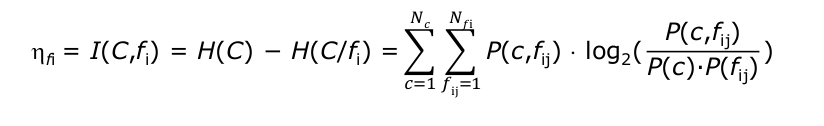
\includegraphics[width=1.0\linewidth]{heuristica}
	\label{fig:heuristica}
	\end{figure}
	
	Donde:
	\begin{itemize}
		\item c = 1, ..., Nc son las clases del problema
		\item 	j = 1, ..., $N_{fi}$ son los valores discretos de $f_i$. Si la característica es
		continua se discretiza en h intervalos (p.ej., h = 10).
		\item 	$P(c,f_{ij})$ es la probabilidad de que un ejemplo del conjunto de
		entrenamiento sea de clase c cuando la variable $f_i$ vale $f_{ij}$.
		\item 	$P(c)$ es la probabilidad de la clase c en el conjunto de entrenamiento
		\item $P(f_{ij})$ es la probabilidad del valor fij en el conjunto de entrenamiento
	\end{itemize}
	

A continuación describiré la implementación de la función heurística en pseudocódigo:
\begin{lstlisting}
heuristica(conjunto_datos, v_heuristico, labels)
begin
  v_heuristico <- rep(conjunto_datos.caracteristicas.length, 0.0)
  n_class <- rep(labels.length, 0)
  
  Para cada vector de caracteristicas i del conjunto de datos
  begin
    Para cada etiqueta j de labels
    begin
      Si i.label == j entonces
        n_class[j] <- n_class[j]+1
    end
  end
  
  Para cada caracteristica i de cualquier vector de caracteristicas del conjunto de datos
  begin
    //Extraigo la caracteristica i de todos los datos
    //del conjunto de datos
    v_auxiliar <- conjunto_datos[,i]
    
    max <- maximo(v_auxiliar)
    min <- minimo(v_auxiliar)
    
    factor <- (max-min)/10.0
    
    matriz <- matrix(labels.lengthx10, 0)
    
    //Esta parte la aclaro redactando mas abajo
    Para cada etiqueta j de labels
    begin
      
      encontrado <- false
      Para k=1 hasta k==10 && !encontrado
      begin
        Si conjunto_datos[,i] <= min+factor*k && j==conjunto_datos[,i].label entonces
          matriz[j,k-1] <- matriz[j,k-1]+1
          encontrado <- true
        
      end
    end
    
    Para cada etiqueta j en labels
    begin
      Para k=0 hasta 10
      begin
        p_i_j <- 0.0
        
        Para h=0 hasta matriz.length
        begin
          p_i_j <- matriz[h,k]+p_i_j
        end
        
        //Probabilidad de ser de clase c en el intervalo
        //discretizado ij
        Si p_i_j==0 entonces
          p_c_f <- 0
        si no
          p_c_f <- matriz[j,k]/p_i_j
          
        //Probabilidad de ser del intervalo discretizado
        p_i_j <- p_i_j/conjunto_datos.length
        
        //probabilidad de ser de una clase
        p_c <- n_class[j]/conjunto_datos.length
        
        Si p_c_f != 0 entonces
          v_heuristico[i] <- v_heuristico[i]+ p_c_f*log2(p_c_f/(p_c*p_i_j))
        si no
          v_heuristico[i] <- v_heuristico[i]+0
          
      end
    end
  end
  
  devolver v_heuristico //por referencia
end

\end{lstlisting}

Redactando un poco el procedimiento. Primero calculo qué número de etiquetas (de cada etiqueta) hay en el conjunto de datos. Después para cada etiqueta i de cualquier vector de características comienzo a calcular su valor heurístico. Para ello calculo cual es el máximo y el mínimo de entre los valores de esta característica para todos los datos. Calculo el factor para discretizar en 10 intervalos y calculo para cada etiqueta cuántas hay en cada intervalo, guardando estas cifras en una matriz que tiene tantas filas como posibles etiquetas y 10 columnas (una por cada intervalo). Después de esto ya incremento el valor heurístico siguiendo la expresión que he dado anteriormente.
\\
\\

En cuanto a la feromona tendremos dos tipos distintos. En mi código lo he representado como 2 arrays distintos. Uno de ellos es la feromona para elegir el número de características (feromona\_n\_car) que la hormiga seleccionará. El otro array será la feromona para la selección de cada una de las características disponibles (feromona\_car).

\section{Algoritmos basados en colonias de hormigas}
Los algoritmos implementados han sido SHMMBL (Sistema de Hormigas Min-Max + Búsqueda Local) y SCHBL (Sistema de Colonia de Hormigas + Búsqueda local). Los aspectos comunes de los dos algoritmos son los siguientes:

\begin{itemize}
	\item Ambos algoritmos usan la misma representación especificada anteriormente

	\item El criterio de parada de ambos algoritmos es no realizar más de 15000 evaluaciones de la función objetivo
	
	\item Ambos usan como función heurística la especificada en el apartado anterior.
	
	\item Los dos algoritmos tendrán los rastros de feromona especificados en el apartado anterior.
	
	\item En los dos algoritmos lanzaremos 10 hormigas. El valor de $\rho$ será 0.2 mientras que $\alpha y \beta$ valdrán 1 y 2 respectivamente.
	
	\item Ambos algoritmos usarán una búsqueda local de una sola iteración para mejorar las soluciones dadas por cada hormiga.
	
	\item En la búsqueda local de una sola iteración que realizo en ambos algoritmos uso la función flip descrita como:
	
	\begin{lstlisting}
	Flip(Solucion, Repetidos)
	begin
	  random <- Random(0, Repetidos.length-1)
	
	  index <- Repetidos[random]
	
	  Si Solucion[index] es true lo cambio a false
	  si no lo cambio a true
	
	  Repetidos-{random}
	
	
	  devolver Solucion
	end
	
	\end{lstlisting}		  			
\end{itemize}


A continuación analizaremos los 2 algoritmos por separado especificando los parámetros concretos para cada algoritmo (los que no son comunes).

\subsection{SCHBL}
En el algoritmo de Sistema de Colonias de Hormigas + Búsqueda Local usaremos los siguientes parámetros:

\begin{itemize}
	\item El valor inicial del rastro de feromona feromona\_car (feromonas para la selección de cada una de las características) será $10^{-6}$.
	
	\item El valor inicial del rastro de feromona feromona\_n\_car (para seleccionar el número de características que seleccionaremos) será $1/N_c$ donde $N_c$ será el número de características de cada vector de características.
	
	\item Para el proceso constructivo usaremos la regla siguiente:
	
	\begin{figure} [H]
	\centering
	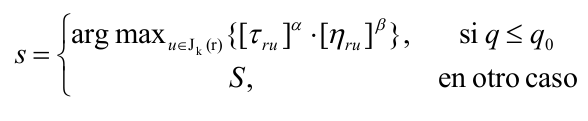
\includegraphics[width=0.7\linewidth]{constructivo}
	\label{fig:constructivo}
	\end{figure}
	
	donde $S$ será una característica cogida simulando una ruleta con una distribución de probabilidad. $q_0$ además es una cota de probabilidad. Si generamos un aleatorio y es menor o igual que $q_0$ entonces cogeremos la característica con más probabilidad, si no, haremos la ruleta.

	\item El parámetro $q_0$ será 0.8.
	
	\item El aporte de feromona a realizar será la tasa de clasificación de la solución dada por la hormiga.
	
	\item El valor de $\varphi $ será 0.2.
	

\end{itemize}

En este algoritmo se realizarán 2 actualizaciones de feromona, una local y otra global. La local se realiza sólo sobre feromona\_car y se realiza cada vez que una hormiga selecciona una característica. Se describe con la expresión siguiente:
\begin{figure} [H]
\centering
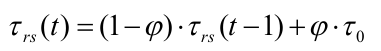
\includegraphics[width=0.5\linewidth]{actualizacionlocal}
\label{fig:actualizacionlocal}
\end{figure}

La actualización global la realizaremos según la mejor solución encontrada hasta el momento y se realizará después de que todas las hormigas hayan hecho su recorrido. La haremos tanto en feromona\_car como en feromona\_n\_car. Seguiremos la siguiente expresión:
\begin{figure} [H]
\centering
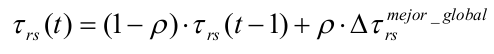
\includegraphics[width=0.5\linewidth]{actualizaciongloba}
\label{fig:actualizaciongloba}
\end{figure}

Donde la aportación de feromona será el valor de la función objetivo (la tasa de clasificación) de la mejor solución encontrada hasta el momento.
\\
\\

Para actualizar feromona\_car, sólo aportaremos feromona en las características que estén seleccionadas por la mejor solución encontrada hasta el momento. Por otro lado para actualizar feromona\_n\_car, contaremos el número de características de la mejor solución y aportaremos feromona sobre la posición correspondiente a este número de características de feromona\_n\_car.

A continuación, la descripción en pseudocódigo del algoritmo:

\begin{lstlisting}
SCHBL(training, solucion, tasa_solucion, heuristica)
begin
  
  //Inicializo las feromonas
  //En la feromona del numero de caracteristicas
  //la posicion i correspondera a coger i+1
  //caracteristicas
  feromona_car <- rep(solucion.length, 1e-6)
  feromona_n_car <- rep(solucion.length, 1/solucion.length)
  
  feromona_n_car_total <- 1.0
  
  evaluaciones <- 0
  
  Mientras que evaluaciones < 15000
  begin
  
    //candidatos sera una matriz que contendra
    //la lista de candidatos para cada hormiga
    //sera un vector de vectores de enteros
    candidatos <- Matrix(10xsolucion.length, 0..solucion.length)
    
    //grafos sera una matriz que contendra
    //cada uno de los vectores solucion dados
    //por cada hormiga. INicialmente inicializadas
    //a false
    grafos <- Matrix(10xsolucion.length, false)
    
    //En n_car guardaremos el numero de caracteristicas
    //que seleccionara la hormiga i-esima y en n_car
    //llevaremos un contador de cuantas caracteristicas
    //ha cogido la hormiga i-esima. Ambos arrays son de
    //tamanio 10
    n_car <- Array(10)
    n_car_seleccionadas <- Array(10)
    
    
    //Pasamos a la seleccion del numero de caracteristicas
    //que cada hormiga cogera. Lo haremos
    //simulando que giramos una ruleta
    
    Para cada hormiga i
    begin
      
      aleatorio <- Random(0,feromona_n_car_total)
      fin <- false
      
      Para cada posicion j de feromona_n_car && !fin
      begin
        aleatorio <- aleatorio-feromona_n_car[j]
        
        Si aleatorio <= 0 entonces
          //La hormiga i cogera j+1 caracteristicas
          n_car[i] <- j+1
          fin <- true
        
      end
    end
          
    
    //Tengo que saber que hormiga cogera mas
    //caracteristicas
    //maximo devuelve el indice del maximo
    n_car_max <- maximo(n_car)
    n_car_max <- n_car[n_car_max]
    
    Para i=0 hasta n_car_max
    begin
      Para cada una de las hormigas j
      begin
      
        //Controlo que la hormiga no elija mas
        //caracteristicas de las que debe
        Si n_car_seleccionadas[j] < n_car[j] entonces
        
          //Inicializo un vector de probs
          probs <- rep(solucion.length, 0.0)
          
          suma_probabilidades <- 0.0
          
          //Recalculo las probabilidades
          //solamente para los candidatos
          //Tengo que tener en cuenta los parametros
          //alpha y beta (2 y 1)
          
          probs[candidatos] <- heuristic[candidatos]*heuristic[candidatos]*feromona_car[candidatos]
          
          suma_probabilidades <- sum(probs)
          
          r <- Rand() //Aleatorio entre 0 y 1
          
          
          Si r <= 0.8 entonces
            //Fase de seleccion de SCH
            //Cojo la caracteristica con mas probabilidad
            mejor_car <- maximo(probs)
            mejor_car <- probs[mejor_car]
            
            grafos[j,mejor_car] <- true
            
            //Aqui realizo la evaporacin local de la
            // feromona
            feromona_car <- 0.8*feromona_car[mejor_car]+0.2*1e-6
            
            //Le quito el elemento mejor_car a candidatos
            candidatos <- candidatos-{mejor_car}
            
          Si no entonces
            //Fase de seleccion de SH
            //Hago una ruleta con una distribucion de
            //probabiliad
            
            aleatorio <- Random(0,suma_probabilidades)
            fin <- false
            index <- -1
            
            Para cada candidato k && !fin
            begin
              aleatorio <- aleatorio-probs[k]
              
              Si aleatorio <= 0 entonces
                index <- k
                fin <- true
                
            end
            
            grafos[j,index] <- true
            
            //Aqui realizo la evaporacin local de la
            // feromona
            feromona_car <- 0.8*feromona_car[index]+0.2*1e-6
                        
            //Le quito el elemento index a candidatos
            candidatos <- candidatos-{index}
          
          n_car_seleccionadas[j]++
          //Fin del if
      end
    end
    
    //Ahora realizaremos unaa busqueda local (con una 
    //sola iteracion) 
    //para cada solucion dada
    //por cada una de las hormigas
    
    Para i=0 hasta 10
    begin
      coste_s_act <- funcion_objetivo(training, grafos[i,])
      evaluaciones++
      
      
      repetidos <- [0...S.length-1]
      
      Mientras que no se mejore y mientras que no se haya generado todo el entorno de S
      begin
        S <- flip(grafos[i,], repetidos) //Con repetidos evitamos repetir dos 			//soluciones de un mismo entorno
        
        coste_S <- funcion_objetivo(training, S)
        evaluaciones++
        
        Si coste_S es mejor que coste_s_act entonces
        //S mejora a Solucion
          grafos[i,] <- S
          coste_solucion <- coste_S
        
      end
        
      Si coste_s_act >= tasa_solucion entonces
        solucion <- grafos[i,]
        tasa_solucion <- coste_s_act
    end
      
    //A continuacion procederemos a la actualizacion 
    //global de la feromona
      
    //Actualizacion de feromona_car
    Para cada componente i de feromona_car
    begin
      fermona_car[i] <- 0.8*feromona_car[i]+0.2*solucion[i]*tasa_solucion
        
    end
      
    //Actualizacion de feromona_n_car
    //Primero cuento cuantas caracteristicas
    //tiene la mejor solucion
      
    mejor_n_car <- 0
      
    Para i=0 hasta solucion.length
    begin
      mejor_n_car <- mejor_n_car+1*solucion[i]
    end
      
    feromona_n_car_total <- 0
      
    Para cada componente i de feromona_n_car
    begin
      feromona_n_car[i] <- 0.8*feromona_n_car[i]+0.2*(mejor_n_car==i+1)*tasa_solucion
        
      feromona_n_car_total <- feromona_n_car_total+feromona_n_car[i]
        
    end
    
  end
  
  devolver solucion y tasa_solucion
  
end
    
\end{lstlisting}

En la implementación, candidatos es un array de arrays de enteros que representan los índices de los vectores de características, donde cada 'fila' i de la matriz (de candidatos) es la lista de candidatos de la hormiga i. Siempre que cojo una característica elimino este candidato de la lista. La búsqueda local la hago con una sola iteración. Además, si mejora, la búsqueda local acaba. Esta condición de parada no estaba muy seguro de si era correcta, pero al final la he dejado. Con el vector repetidos me aseguro de que ya se ha explorado todo el entorno de la solución (o no). La función flip ya la he explicado en pseudocódigo anteriormente.



\subsection{SHMMBL}

En este algoritmo usaremos los siguientes parámetros y decisiones:

\begin{itemize}
	\item El valor inicial de feromona será $\tau_{max}=C(S_{aleatoria})/\rho$ para feromona\_car (que será la cota máxima de feromona) y la cota inferior de feromona será $\tau_{max}/500$.
	
	\item Cada vez que encontremos una solución que supere a la mejor global, actualizaremos $\tau_{max}=C(S_{mejor})/\rho$ y $\tau_{min}=\tau_{max}/500$.
	
	\item En este algoritmo sólo se hará actualización de la feromona de forma global (no habrá actualización local).
	
	\item Para feromona\_n\_car no he usado las cotas de feromona.
	
	\item En el proceso constructivo se usa la regla de selección de SH. Se hace una ruleta con una distribución de probabilidad y elegimos según esa ruleta.
\end{itemize}

La actualización de este algoritmo se basa en la regla:
\begin{figure} [H]
\centering
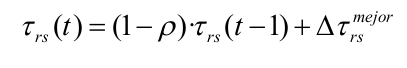
\includegraphics[width=0.7\linewidth]{actualizacionshmml}
\label{fig:actualizacionshmml}
\end{figure}

es decir, para actualizar la feromona sólo nos fijaremos en la mejor solución encontrada hasta el momento. Además, como he dicho anteriormente, tendremos una cota de feromona con la que haremos que la feromona no sea ni demasiado alta ni demasiado baja, permitiendo así algo más de diversidad. Además, estas cotas se irán actualizando según vayamos encontrando mejores soluciones globales, como he explicado anteriormente.
\\
\\

La descripción en pseudocódigo es la siguiente:
\begin{lstlisting}
SHMMBL(training, solucion, tasa_solucion, heuristica)
begin

  //Primero generamos una solucion aleatoria
  solucion <- generar_solucion_aleatoria(solucion, solucion.length)
  tasa_solucion <- funcion_objetivo(training,solucion)
  
  //Inicializo las feromonas
  //En la feromona del numero de caracteristicas
  //la posicion i correspondera a coger i+1
  //caracteristicas
  
  max_feromona <- tasa_solucion/0.2
  min_feromona <- max_feromona/500.0
  
  feromona_car <- rep(solucion.length, max_feromona)
  feromona_n_car <- rep(solucion.length, 1/solucion.length)
  
  feromona_n_car_total <- 1.0
  
  evaluaciones <- 0
  
  Mientras que evaluaciones < 15000
  begin
  
    //candidatos sera una matriz que contendra
    //la lista de candidatos para cada hormiga
    //sera un vector de vectores de enteros
    candidatos <- Matrix(10xsolucion.length, 0..solucion.length)
  
    //grafos sera una matriz que contendra
    //cada uno de los vectores solucion dados
    //por cada hormiga. INicialmente inicializadas
    //a false
    grafos <- Matrix(10xsolucion.length, false)
   
    //En n_car guardaremos el numero de caracteristicas
    //que seleccionara la hormiga i-esima y en n_car
    //llevaremos un contador de cuantas caracteristicas
    //ha cogido la hormiga i-esima. Ambos arrays son de
    //tamanio 10
    n_car <- Array(10)
    n_car_seleccionadas <- Array(10)
  
  
    //Pasamos a la seleccion del numero de caracteristicas
    //que cada hormiga cogera. Lo haremos
    //simulando que giramos una ruleta
  
    Para cada hormiga i
    begin
  
      aleatorio <- Random(0,feromona_n_car_total)
      fin <- false
  
      Para cada posicion j de feromona_n_car && !fin
      begin
        aleatorio <- aleatorio-feromona_n_car[j]
  
        Si aleatorio <= 0 entonces
        //La hormiga i cogera j+1 caracteristicas
          n_car[i] <- j+1
          fin <- true
  
      end
    end
  
  
    //Tengo que saber que hormiga cogera mas
    //caracteristicas
    //maximo devuelve el indice del maximo
    n_car_max <- maximo(n_car)
    n_car_max <- n_car[n_car_max]
  
    Para i=0 hasta n_car_max
    begin
      Para cada una de las hormigas j
      begin
  
        //Controlo que la hormiga no elija mas
        //caracteristicas de las que debe
        Si n_car_seleccionadas[j] < n_car[j] entonces
  
        //Inicializo un vector de probs
          probs <- rep(solucion.length, 0.0)
  
          suma_probabilidades <- 0.0
  
          //Recalculo las probabilidades
          //solamente para los candidatos
          //Tengo que tener en cuenta los parametros
          //alpha y beta (2 y 1)
  
          probs[candidatos] <- heuristic[candidatos]*heuristic[candidatos]*feromona_car[candidatos]
  
          suma_probabilidades <- sum(probs)
  

          //Fase de seleccion de SH
          //Hago una ruleta con una distribucion de
          //probabiliad
  
          aleatorio <- Random(0,suma_probabilidades)
          fin <- false
          index <- -1
  
          Para cada candidato k && !fin
          begin
            aleatorio <- aleatorio-probs[k]
  
            Si aleatorio <= 0 entonces
              index <- k
              fin <- true
  
          end
  
          grafos[j,index] <- true
  
          //Le quito el elemento index a candidatos
          candidatos <- candidatos-{index}
  
          n_car_seleccionadas[j]++
          //Fin del if
      end
    end
  
    //Ahora realizaremos unaa busqueda local (con una 
    //sola iteracion) 
    //para cada solucion dada
    //por cada una de las hormigas
  
    Para i=0 hasta 10
    begin
      coste_s_act <- funcion_objetivo(training, grafos[i,])
      evaluaciones++
  
  
      repetidos <- [0...S.length-1]
  
      Mientras que no se mejore y mientras que no se haya generado todo el entorno de S
      begin
        S <- flip(grafos[i,], repetidos) //Con repetidos evitamos repetir dos 			//soluciones de un mismo entorno
  
        coste_S <- funcion_objetivo(training, S)
        evaluaciones++
  
        Si coste_S es mejor que coste_s_act entonces
          //S mejora a Solucion
          grafos[i,] <- S
          coste_solucion <- coste_S
  
      end
  
      Si coste_s_act >= tasa_solucion entonces
        solucion <- grafos[i,]
        tasa_solucion <- coste_s_act
        
        //Actualizo las cotas de feromona
        max_feromona <- tasa_solucion/0.2
        min_feromona <- max_feromona/500
    end
  
    //A continuacion procederemos a la actualizacion 
    //de la feromona
  
    //Actualizacion de feromona_car
    Para cada componente i de feromona_car
    begin
      fermona_car[i] <- 0.8*feromona_car[i]+solucion[i]*tasa_solucion
      
      Si feromona_car[i] > max_feromona entonces
        feromona_car[i] <- max_feromona
      Si no si feromona_car[i] < min_feromona entonces
        feromona_car[i] <- min_feromona
    end
  
    //Actualizacion de feromona_n_car
    //Primero cuento cuantas caracteristicas
    //tiene la mejor solucion
  
    mejor_n_car <- 0
  
    Para i=0 hasta solucion.length
    begin
      mejor_n_car <- mejor_n_car+1*solucion[i]
    end
  
    feromona_n_car_total <- 0
  
    Para cada componente i de feromona_n_car
    begin
      feromona_n_car[i] <- 0.8*feromona_n_car[i]+*(mejor_n_car==i+1)*tasa_solucion
  
      feromona_n_car_total <- feromona_n_car_total+feromona_n_car[i]
  
    end
  
  end
  
  devolver solucion y tasa_solucion
  
end
  
\end{lstlisting}

\section{Experimentos y análisis}
A continuación las gráficas de resultados para cada algoritmo:
\begin{figure} [H]
\centering
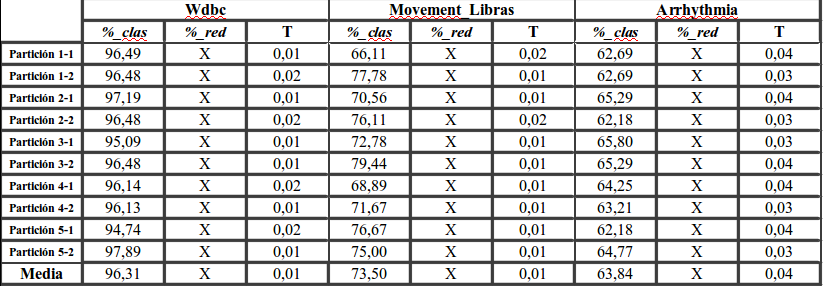
\includegraphics[width=1.0\linewidth]{3NN}
\caption{Resultados para 3NN}
\label{fig:3NN}
\end{figure}

\begin{figure} [H]
\centering
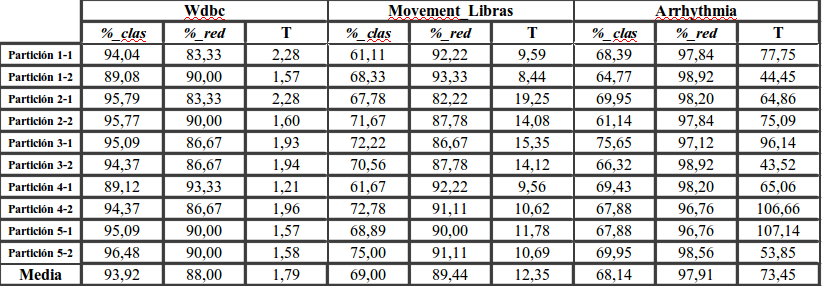
\includegraphics[width=1.0\linewidth]{SFS}
\caption{Resultados para SFS}
\label{fig:SFS}
\end{figure}

\begin{figure} [H]
\centering
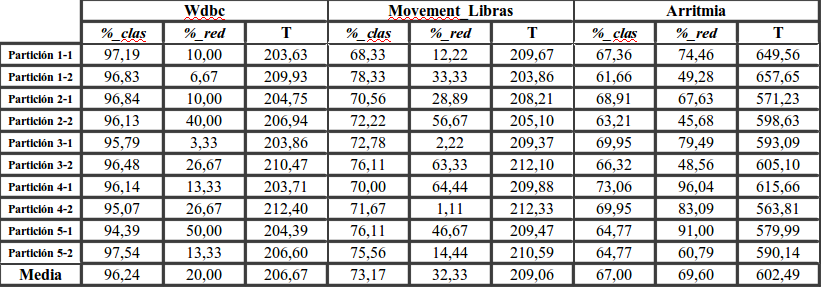
\includegraphics[width=1.0\linewidth]{SCHBL}
\caption{Resultados para SCHBL}
\label{fig:SCHBL}
\end{figure}

\begin{figure} [H]
\centering
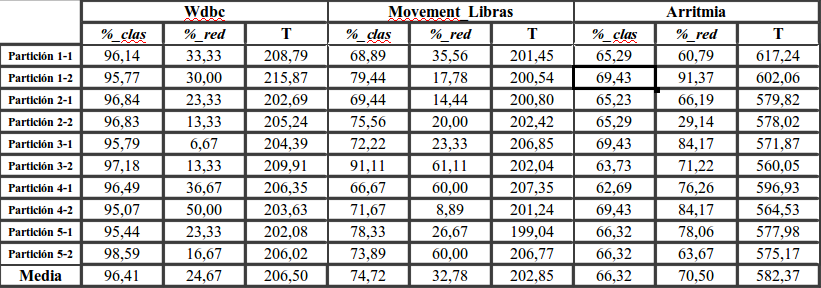
\includegraphics[width=1.0\linewidth]{SHMMBL}
\caption{Resultados para SHMMBL}
\label{fig:SHMMBL}
\end{figure}

Como vemos en la base de datos de Wdbc, ambos algoritmos de hormigas mejoran los resultados del algoritmo de comparación (SFS). En cambio, en el 3NN, obtenemos mejores resultados que en SCHBL. Esto podría deberse a que esta base de datos apenas tiene características ruidosas. SFS tiene una tasa de clasificación muy baja en comparación con los dos algoritmos basados en el comportamiento de hormigas. Como ya he dicho, esta base de datos por lo visto es poco ruidosa. EN SFS tenemos una tasa de reducción del 88\% por lo que hemos quitado muchas características y posiblemente algunas importantes. En las dos metaheurísticas reducimos el vector de características bastante menos, y por esto podría ser por lo que nos da mucho mejores resultados. El hecho de que en SHMMBL de resultados algo mejores en esta base de datos podría deberse a que este algoritmo intensifica mucho sobre la mejor solución (más que SCHBL), por lo que probablemente obtenga soluciones mejores.
\\
\\
En la segunda base de datos también las dos metaheurísticas mejoran los resultados de SFS. También puede deberse a una menor tasa de reducción, lo que nos puede hacer pensar a que esta base de datos es, como la anterior, poco ruidosa. Podemos confirmar esta teoría al ver el resultado de 3NN, que sin reducir ninguna característica (obviamente) mejora también SFS. SHMMBL también mejora a todos los algoritmos, y se podría deber a, como he comentado antes, la intensificación sobre las buenas soluciones. En cuanto a los tiempos, esta base de datos tarda menos que la primera a pesar de tener más características, y podría deberse a que tiene menos instancias.
\\
\\
En la tercera base de datos cambia el contexto. Arrhythmia es una base de datos con gran número de características y probablemente mucho ruido. Esto lo confirma el hecho de que SFS obtenga mejor tasa de clasificación que 3NN. SFS también obtiene mejores resultados que los dos algoritmos implementados. Al comenzar a explorar desde una solución 'vacía', elimina muchas más características (cae en un óptimo local pronto) y muy probablemente muy ruidosas. Entre los dos algoritmos implementados, SHMMBL presenta una tasa de clasificación media algo menor que SCHBL y creo que se debe a que SCHBL permite más diversificación que SHMMBL, que intensifica más sobre las buenas soluciones. El hecho de que diversifique más es bueno cuando los entornos de búsqueda son tan amplios como en esta base de datos.

\end{document}